\section{Place Recognition Algorithm}
\label{sec:chap_slam_algo}

While there are quite a few articles presenting place recognition algorithms using different sensors (e.g. cameras, \gls*{gps}), the literature of such algorithms based solely on \gls*{3d} data is limited. For our place recognition analysis, we choose to evaluate on our datasets the state-of-the-art algorithm (at the time of the experiments) developed by \citet{Steder2011b}. The full details of the technique are presented in the article. However for the sake of this document, we will first describe some fundamental concepts used for place recognition in Section~\ref{ssec:chap_slam_basics} and then we will give an overview of the Steder algorithm itself in Section~\ref{ssec:chap_slam_algo}.


\subsection{Fundamental Concepts}
\label{ssec:chap_slam_basics}

The following subsection is an introduction to the basic concepts necessary for understanding the place recognition algorithm, which will be presented in Section~\ref{ssec:chap_slam_algo}. Conventional methods for representing and comparing \gls*{3d} acquisitions will be presented. 

\subsubsection{Feature Keypoints and Descriptors}
\label{ssub:feature_keypoints_and_descriptors}

The first step in determining whether or not a place has been visited before by the robot, is to convert the sensor data into a format that is more convenient for identification. The generally adopted representation is a vector of real numbers, called descriptor. This mathematical representation is usually more compact than the original data and should try to capture significant characteristics.

A descriptor can be global, meaning that it tries to capture information about the whole sample, or local, meaning that it does the same but only for a specific subregion of the sample. When using local descriptors, it is first required to determine the keypoints around which the descriptors will be extracted. These keypoints can be at pre-determined and fixed locations (e.g. division in a simple grid) or selected using more refined algorithms. A common practice for the latter is to choose keypoints in so-called interesting which are regions of high gradient (e.g. edges, corners), as these region generally contains more information than smooth surfaces. Note that for simplicity, we might use the term \textbf{features} as a more general term for keypoints and their respective descriptors in the remainder of this document.

The concepts of keypoints and descriptors first originated from the computer vision literature, but they have recently been adapted for \gls*{3d} data. Some popular examples of features for both type of data are shown in Table~\ref{tab:features_examples}. Note that some algorithms propose solutions for both keypoints detection and descriptors (e.g. SIFT, NARF). However it is not mandatory to use them together as any combination is generally valid. While all features are different, they were all developed with the same goals in mind:
\begin{itemize}[label=$\bullet$,noitemsep,topsep=0pt]
    \item Distinctiveness: each feature should be easily differentiable with respect to othes.
    \item Repeatability: the feature values should be stable under changes including:
        \begin{itemize}[label=$\circ$,noitemsep,topsep=0pt]
            \item Transformations: rigid transformation for point clouds and projective transformation for images, but also changes in the pose of the objects and/or the viewpoint.
            \item Noise: small variations in measurements (range/intensity) and occasional erroneous values (points/pixels).
            \item Resolution: the number of points or pixels representing a given area.
        \end{itemize}
\end{itemize}


\subsubsection{Range Image and NARF Feature}
\label{ssub:NARF Features and Range Image}

In this subsection, we will present the NARF keypoints and descriptors, as well as the \gls*{3d} data representation on which they rely: the range image. We will see that the place recognition algorithm, presented in Section~\ref{ssec:chap_slam_algo}, relies on this \gls*{3d} representation to determine a matching score between scans.

Range images represent a \gls*{3d} data point by a pixel position (i.e x and y) and a range value. Note that the position of the pixel actually represents a horizontal and vertical angular position. For an omnidirectional \gls*{lidar} scan, the corresponding range image is a spherical projection of the points from the center of the sensor. Range images can be better defined by the constraints they must meet to be valid. 

Firstly, converting a \gls*{3d} scan into a range image requires the acquisition to originate from a single view point and to have a single range value per pixel. It is therefore not possible to use point clouds acquired with multi-echoes \gls*{lidar}s or produced by merging multiple scans. Fortunately, the latter constraint is met in our datasets.

Secondly, all pixel from the range image must have a value. Since \gls*{lidar}s have a minimal and a maximal range, the data points outside this interval are ignored. Similarly, when a laser beam hit a highly absorbing or reflecting surface, the sensor will not get any return. When such missing data points cause pixels of the range image to have no value, the latter are considered as far range (i.e. the maximum range of the sensor). 

Finally, the resolution has to be adjusted so that each pixel of the resulting range image covers the same angular resolution vertically and horizontally. The image being discretized in pixels, the values of these can either be a weighted average of the laser beam ranges, or the value of the smaller range within his area, depending on the user preference. Examples of range images can be seen in Figure~\ref{fig:chap_slam_range}.

The converted scans have a dense and uniform representation that can be advantageously processed like grayscale images. Using these range images, NARF features were designed to be able to differentiate edges that are part of the boundary of objects as opposed to edges that are produced by occlusions. This distinction is not possible using point clouds directly. This will be particularly useful in our context of complex environments such as forest, where edges caused by occlusions can generate meaningless features. These meaningless features turn leads to a poor representation of the environment, which can reduce the place recognition performance. \todo{Add a figure with a point cloud and the corresponding range image and point out the false edges in the point cloud (caused by occlusion)}


\begin{figure}[H]
    \centering
    \subfloat[]{\label{fig:range_building}}{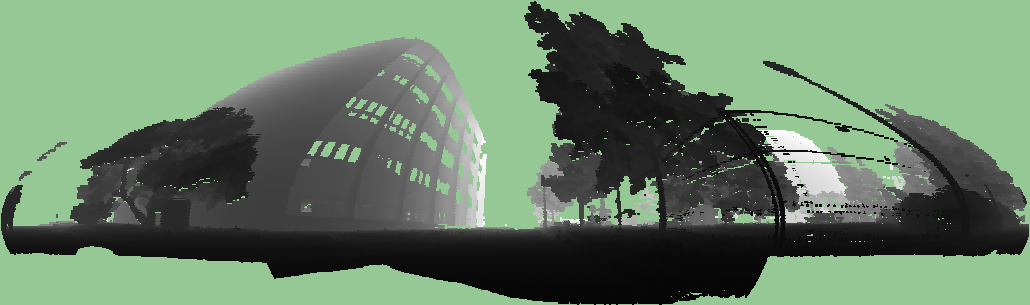
\includegraphics[width=0.995\linewidth]{img/chap_slam/range_building01.png}}\\
    \subfloat[]{\label{fig:range_forest}}{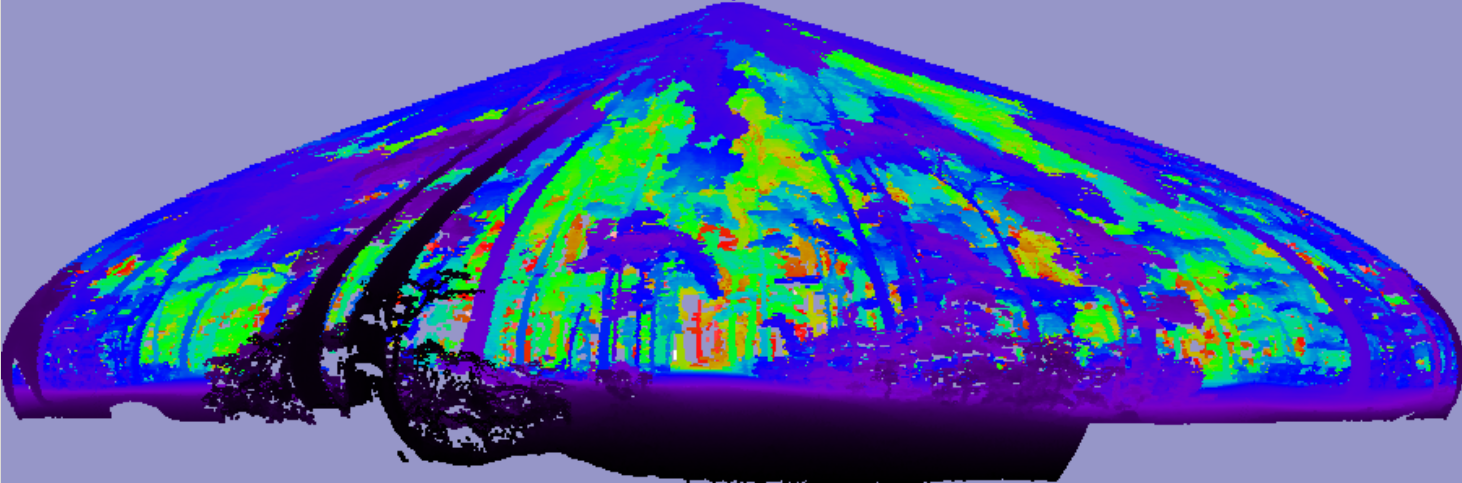
\includegraphics[width=0.995\linewidth]{img/chap_slam/range_forest01.png}}
    \caption{Examples of range images for the structured dataset \protect\subref{fig:range_building} and the unstructured dataset \protect\subref{fig:range_forest}. Note that the objects look distorted due to the projection on the plane and that the background color corresponds to the areas without laser return.}
    \label{fig:chap_slam_range}
\end{figure}

\subsubsection{Scans Comparison}
\label{ssub:scans_comparison}

The last item to be discussed in this subsection is the method used to compare two scans. Since a descriptor contains a predefined sequence of values representing the underlying data, two descriptors with very similar corresponding values should also represent similar entities (i.e. objects). Consequently, similarity between descriptors are generally computed using a simple distance metric (e.g. Euclidean distance, cosine distance).

The comparison between two scans using global descriptors is usually computationally inexpensive. Indeed, a single descriptor has to be computed for each scan and the comparison between two of them requires the computation of only one distance metric. Also note that for global descriptors, there is no such thing as keypoints and the geometric information is intrinsically included in the descriptor itself. A major drawback of such comparison approach is the high sensitivity to local changes of the environment, which may for example be caused by dynamic objects.

On the contrary, scans comparison based on local descriptors require more computation. Besides having to calculate several keypoints and associated descriptors for each scan, a method must be chosen to compare two scans over all features. In addition, the geometric relation between features provides important information about scans and may be considered, but this also requires more processing. Fortunately, using local features generally yield more robust results regarding local changes and also provides more comparison flexibility for the user. We will see examples of techniques for comparing scan using local features.

A first approach to compare \gls*{3d} scans consists in finding local descriptors correspondences between the scans and use these correspondences to check if there is a valid transformation that aligns the scans. The vectors of real numbers representing the features (i.e. the descriptors) will never be exactly the same from one scan to another, but a simple solution is to use the nearest neighbor as the correspondence. Unfortunately, this does not take into account the fact that several descriptors may have no valid match due to background clutter or change in the view point. \cite[Section 7.1]{Lowe2004} describes how to remove most of the false matches by comparing the distance of the closest neighbor to that of the second-closest neighbor. The intuition is that this second best match is an incorrect one and using this ratio, only matches that have the closest neighbor significantly closer than the closest next match will be used, therefore improving reliability.

Once the corresponding descriptors between two scans have been identified, they are used to determine if there is a valid rigid \gls*{3d} transformation that align the underlying keypoints. This step also requires a criteria on the number (or ratio) of features correctly aligned, thereby identifying the scans as originating from the same place or not. This is generally achieved using the RANSAC algorithm~\cite{Fischler1981}. This first comparison technique is computationally expensive, but is also very discriminative. Additionally, it provides relative pose between scans, which is not possible using global descriptors or the next method that we will present. The relative pose can, for example, be used to determine odometry or create a map. Figure~\ref{fig:chap_slam_features_correspondences} shows keypoints from two scans of our dataset, as well as examples of correspondences.

A second solution, that speed up comparison when searching for potential matches between scans, is to represent the set of features of each scan by a \gls*{bow}~\citep{salton1983mcgill}. The concept of \gls*{bow} was first used for documents classification. In this context, \gls*{bow} represented a document by a vector of occurrence counts of a vocabulary without taking into account their ordering. In our case, the descriptors are made up of real numbers which allows for an infinity of them and therefore they cannot be used directly as words. The solution to this problem is to use a clustering algorithm such as k-means~\citep{MacQueen1967} to create groups that will represent words, a process known as quantization. An advantage of using k-means is that it is an unsupervised algorithm, meaning that no manual labeling effort is required. Because the \gls*{bow} approach avoids having to compare all potential feature correspondences between the scans, it significantly reduces the processing time. On the other hand, this method removes all information regarding to geometric configuration of keypoints in the scans, which might induce unwanted aliasing. This is a rather general representation with for which the comparison is relatively fast to compute. Note that the vocabulary is generally created in advance using a large collection of local descriptors gathered under similar conditions. 

The chosen place recognition method will depends on several factors such as the available hardware resources, the desired processing time and the required reliability of the results. Using features correspondences along with geometric check is more computationally expensive than using the \gls*{bow} approach, but results are also more reliable. However, we will see in Section~\ref{ssec:chap_slam_algo} that it is possible to take advantage of the combined use of these methods. 

\begin{figure}[H]
    \centering
    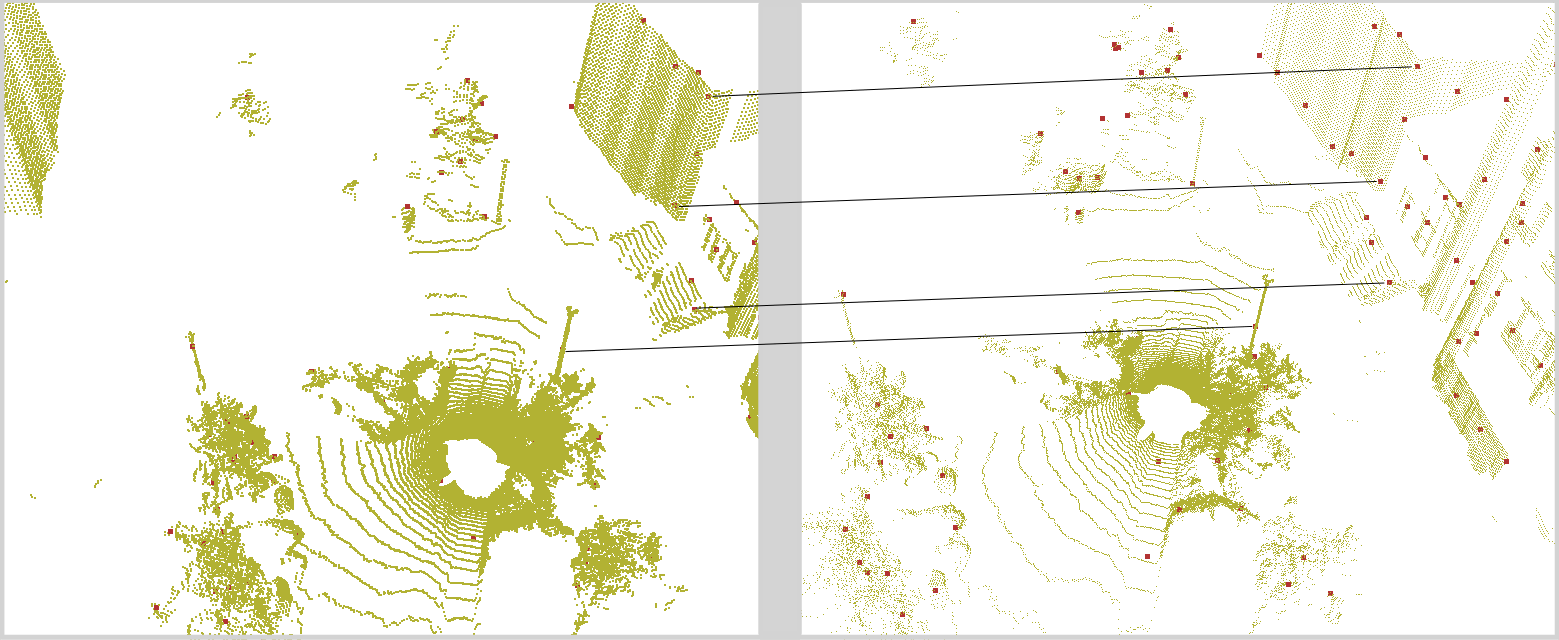
\includegraphics[width=0.995\linewidth]{img/chap_slam/features_line.png}\\
    \caption{Examples of NARF keypoints (red squares) found for two different scans of the structured dataset. Black lines illustrate examples of valid correspondences found across scans. These NARF keypoints show stability under changes, such as viewpoint, noise and resolution.}
    \label{fig:chap_slam_features_correspondences}
\end{figure}


\subsection{Overview of the Algorithm}
\label{ssec:chap_slam_algo}

For their experiments, Steder et al. drive a rover equipped with a \gls*{lidar} in a given environment to gather a set of scans. They refer to it as the scans database, which acts as a representation of all known places. The robot can later navigate in the same area, acquire a new scan and try to determine if it corresponds to a previously visited place based on the database scans. 

In the original version of the algorithm (\cite{Steder2010}), they compare a newly acquired scan against all scans from the database using NARF features correspondences. These features encode a full \gls*{3d} pose, allowing to determine the transformation that align two scans based on a single features correspondence. This mean that there is as many candidate transformations as there are features correspondences between a newly acquired scan and a scan from the database. Using series of rules, a score is assigned to each transformation. This score reflects the system belief of this transformation to be an actual match. Advantageously, this means that the algorithm not only indicates whether two scans represent the same place, but also what is the relative pose between them.

Although this technique yield high recognition rates, it requires to compute a score for all candidate transformations (i.e. features correspondences) between the new scan and all scans from the database. This process is too computationally expensive for real time application. An enhanced version of the algorithm, that we used for our experiments, was presented in~\cite{Steder2011b}. To improve processing time, they select only pairs of scans (i.e. the new scan and a scan from the database) with the highest \gls*{bow} similarity for the scoring step. Also, because the first version of the algorithm yield poor result in area with less distinctive structure, they added a self-similarity analysis. Using the score of the best non-identity transformation of a scan with respect to itself, they adjust the score with respect to the other scans, thereby reducing the number of false positive. Finally, they modified the NARF features to be invariant to rotations. Algorithm~\ref{alg:chap_slam_overview} present a high level pseudocode of the general scan matching process. Note that for the experiments, we used a \textit{C++} implementation developed by Bastian Steder.

\begin{algorithm}
    \begin{algorithmic}[1]
        \INPUT
        \Statex $scanDatabase$ : the complete database of previous scans (range images)
        \Statex $newScan$ : the new scan to be processed
        \OUTPUT
        \Statex $potentialMatches$ : set of (scanDatabase potential match for the newScan, best relative transformation, transformation score)
        \Statex

        \Function{findPotentialMatches}{$scanDatabase$, $newScan$}
        \State $allBowDescriptors \gets \textsc{calculateAllDescriptorsForBagOfWords}(scanDatabase)$ \label{alg:bow_beginning}
        \State $dictionary \gets \textsc{createDictionaryForBagOfWords}(allBowDescriptors)$
        \State $newScanBow \gets \textsc{computeBagOfWords}(newScan, dictionary)$ \Comment{Keep scan reference} \label{alg:create_bow}
        \State \State $initSimilarities \gets \emptyset$ \Comment{Set of (scan reference, initial similarity score)}
        \ForAll{$scan \in scanDatabase$}
        \State $scanBow \gets \textsc{computeBagOfWords}(scan, dictionary)$
        \State $initSimilarities.append(\textsc{getInitSimilarity}(scanBow, newScanBow))$ \label{alg:init_similarities}
        \EndFor
        \State $sortedSimilarities \gets \textsc{sortByScore}(initSimilarities)$ \label{alg:bow_end}

        \State
        \State $potentialMatches \gets \emptyset$, $i \gets 1$ \label{alg:correspondences_beginning}
        \State $newScanFeatures \gets \textsc{getScanFeatures}(newScan)$  \Comment{Each feature encodes the 3D pose} \label{alg:features_1}
        \While{$time \leq timeout$ \textbf{and} $i \leq |scanDatabase|$} \label{alg:timeout}
        \State $scan \gets \textsc{getScan}(sortedSimilarities_i)$
        \State $scanFeatures \gets \textsc{getScanFeatures}(scan)$ \Comment{Each feature encodes the 3D pose} \label{alg:features_2}
        \State $sortedMatches \gets \textsc{getSortedFeatureMatches}(scanFeatures, newScanFeatures)$ \label{alg:ordered_matches}

        \State
        \State $j \gets 1$, $bestTransfoScore = -\infty$, $bestTransfo \gets null$
        \While{$j \leq |sortedMatches|$ \textbf{and} $j \leq 2000$} 
        \State $transfo,score \gets \textsc{computeMatchTransfoAndScore}(sortedMatches_j)$ \label{alg:transfo_score}
        \If{$score \geq scoreAcceptanceThreshold$ \textbf{and} $score \geq bestTransfoScore$}
        \State $bestTransfoScore \gets score$
        \State $bestTransfo \gets transfo$
        \EndIf
        \State $j \gets j + 1$
        \EndWhile

        \State
        \If{$bestTransfo \neq null$}
        \State $potentialMatches.append(scan, bestTransfo, bestTransfoScore)$
        \EndIf

        \State
        \State $i \gets i+1$
        \EndWhile \label{alg:correspondences_end}

        \State
        \State \Return{$potentialMatches$}
        \EndFunction
    \end{algorithmic}

    \caption{High Level Place Recognition Process}
    \label{alg:chap_slam_overview}
\end{algorithm}

In Algorithm~\ref{alg:chap_slam_overview}, NARF features are computed twice for each scan. The \gls*{bow} preprocessing from line~\ref{alg:bow_beginning} to~\ref{alg:bow_end} uses a set of feature parameters while the correspondences scoring from line~\ref{alg:correspondences_beginning} to line~\ref{alg:correspondences_end} use a different set of parameters. Table~\ref{tab:chap_slam_narf_parameters} shows the feature parameters used for those two cases. Authors explain that: \enquote{For the BoW approach a high number of features describing small parts of the environment is most useful\dots However, when matching a new query [scan] $z*$ against D [the database], a smaller number of more distinctive features is needed}.

\begin{table}[H]
    \centering
    \begin{tabular}{@{}lll@{}}
        \toprule
        \textbf{Parameters}  & \textbf{Values for \gls*{bow}} & \textbf{Values for the correspondences scoring} \\
        \hline
        Max. feature counts & 2000                          & 200                                \\
        Descriptor size     & 36                            & 36                                 \\
        Support size        & 1/10 avg. range               & 1/5 avg. range                     \\
        \bottomrule
    \end{tabular}
    \caption{The set of NARF parameters used for the \gls*{bow} preprocessing and the correspondences scoring. Note that the support size is a proportion of the average range of all points in the database.}
    \label{tab:chap_slam_narf_parameters}
\end{table}

The descriptors produced for the \gls*{bow} are used by the \textsc{createDictionaryForBagOfWord} function, which create 200 words (i.e clusters) using k-means. The output dictionary is used to create a \gls*{bow} representation for each scan. Based on this representation, all scans from the database are stored in ascending order, according to their Euclidean distance from the input scan (line~\ref{alg:init_similarities}). Scans with a small distance between them are more likely to originate from the same place and will be processed first during the next step. This order is important because of the timeout (line~\ref{alg:timeout}) that might prevent last scans to be processed.

The features created using the set of parameters for correspondences scoring are used to find potential transformations between each database scan and the input scan. As indicated earlier, each NARF feature encodes its full 3D pose, therefore a single features match allows to determine the transformation that align the two scans. This mean that there are up to 2000 transformations to be tested for each scan from the database. To determine the corresponding features, all pairs of features (one from the processed database scan and one from the input scan) are then ordered by ascending order according to their Manhattan distance in the space of descriptors. Again, descriptors with a small distance between them are more similar and therefore more likely to be valid matches and are therefore prioritized for the scoring process.

Although the candidate transformation scoring process is not detailed (line~\ref{alg:transfo_score}), it is an important part of the place recognition framework that we will briefly describe here. As explained in Section~\ref{ssec:chap_slam_basics}, range images are linked to the \gls*{lidar} sensor model. Each pixel represent the range from the origin of the sensor to the target for a specific angular position. Given that the input scan ($z^*$) have already been aligned with the database scan ($z^i$), one can easily determine where the pixel $p^*$ from $z^*$ will fall into $z^i$, as well as the range value it should have. Let $r^*$ be the range of the processed point in $z^*$ and $r^i$ the range of the corresponding point in $z^i$. A score representing how good $r^*$ is explained by $r^i$ can be computed according to different scenarios presented in Table~\ref{tab:chap_slam_scoring_scenarios}.
This scoring process is applied to all validation points and the final score for the candidate transformation is a function of those individual point scores. To avoid a small error in the transformation to cause low score, they not only consider the exact matching points, but also neighbors in small pixel radius. Finally, note that the set of validation point is a subsample of points evenly covering the 3D space, since using all points from the input scan would be too expensive to compute.

\begin{table}[H]
    \centering
    \begin{tabular}{@{}p{0.17\textwidth}p{0.54\textwidth}p{0.23\textwidth}@{}}
        \toprule % Observation = database, Prediction = input scan
        \textbf{Ranges relation}         & \textbf{Explanation}                                                                                                    & \textbf{Effect on the score} \\
        \hline                           
        $|r^i - r^*| < \Delta r_{max}$   & The difference between $r^i$ and $r^*$ is within the confidence range. This is most likely a valid correspondence.      & Reward $\propto 1-\frac{|r^i-r^*|}{\Delta r_{max}}$ \\
        $r^i - r^* > \Delta r_{max}$     & The range of the pixel from the database scan is larger than the corresponding pixel from the input scan. This could be caused by a dynamic or partially transparent obstacle, but this is more likely caused by a wrong transformation. & High penalty \\
        $r^i - r^* < -\Delta r_{max}$    & The range of the pixel from the database scan is smaller than the range of the corresponding pixel from the input scan, leading to two subcases : & \\
                                         & 1) A known obstacle in the database scan hides the pixel from the input scan.                                           & Low penalty \\
                                         & 2) The pixel does not exist in the input scan. This could be caused by an unseen or dynamic obstacle, but it is more likely caused by a wrong transformation.       & High penalty \\
        $\nexists : r^i \correspond r^*$ & The pixel from the input scan ends up outside of the database scan limit (i.e. there is no reference for this point).   & Low penalty \\
        $r^i \ge MAX$                    & The range of the pixel from the database scan is larger or equal to the sensor maximum reading range, leading to two subcases : & \\
                                         & 1) Based on the value of the input scan pixel, the corresponding pixel of the database should be closer to the sensor.  & High penalty \\
                                         & 2) The pixel of the database scan moved away from the sensor and could possibly be out of range.                        & Medium penalty \\
        \bottomrule
    \end{tabular}
    \caption{A summary of the different scenarios for scoring corresponding pixels of the range images. The range of the pixel from the input scan is $r^*$ and the range of the corresponding pixel from the database scan is $r^i$. Note that, $\Delta r_{max}$ is a positive value representing the maximum difference in range between the pixels to be considered as a valid correspondence and $MAX$ is the maximum range for the given sensor.}
    \label{tab:chap_slam_scoring_scenarios}
\end{table}

This concludes the general overview of the place recognition algorithm. In Section~\ref{sec:chap_slam_results}, we will explain how we use it to compare the impact of different environments on the recognition performance.
